\chapter{Video}
\renewcommand{\kapitelautor}{Autor: Kerstin Schön}
\section{Technik}
\subsection[Auflösung]{Auflösung\protect\footnote{\label{}vgl. Jörg Jovy, 2017, S. 109f.}}
Bei der Auflösung wird heutzutage unter SD, HD (2k), Digital Cinema (2k) und UHD (4k/8k) unterschieden. SD bedeutet Standard Definition und dominierte früher das Fernsehen. Heutzutage ist der Standard nicht mehr Standard Definiton, sondern High Definition. Obwohl bei Smartphones, TV-Geräten und Kameras schon Full-HD, also 1920 x 1080 px, der Vorreiter ist, wird zumindest im deutschen Fernsehen noch im normalen HD Format, also 1280 x 720 px, ausgestrahlt. 
\subsection[Bildrate]{Bildrate\protect\footnote{\label{}vgl. Jörg Jovy, 2017, S. 111f.}}
Seit 1967 wird im deutschen Fernsehen mit dem sogenannten PAL Format (=Phase Alternative Line) gesendet. Im PAL Format werden 25 Bilder pro Sekunde oder 50 Halbbilder pro Sekunde gesendet. Jedoch herrscht in den USA nicht das PAL Format, sondern das sogenannte NTSC Format (=National Television Systems Committee), welches 30 Vollbilder pro Sekunde oder 60 Halbbilder pro Sekunde sendet. Diese unterschiedlichen Bildraten sind der Tatsache geschuldet, da in Europa eine Wechselspannungsfrequenz von 50Hz herrscht, und in den USA eine von 60Hz.
\subsection[Farbraum]{Farbraum\protect\footnote{\label{}vgl. Jörg Jovy, 2017, S. 112f.}}
Rot, Grün und Blau sind die drei Grundfarben des RGB Farbraums. Aus den drei Grundfarben bilden sich alle anderen Farben, die im RGB Farbraum möglich sind, was man RGB-Farbmischung nennt. "Bei einer 8-Bit-Codierung pro Farbe stehen 256 verschiedene Farbwerte zur Verfügung. Aus der Mischung ergeben sich theoretisch 16,78 Mio. verschiedene Farbwerte (= 256 x 256 x 256)."\footnote{\label{}vgl. Jörg Jovy, 2017, S. 113} Schwarz enthält keine Farbinformation von den drei Grundfarben, wohingegen Weiß die Mischung aller drei Grundfarben ist. Der Farbraum des HD Standards ist RGB oder sRGB. Es kann nur die Farbinformation dargestellt werden, die sich auch in dem verfügbaren Farbraum befinden. 
\begin{figure}[H]
	\centering
	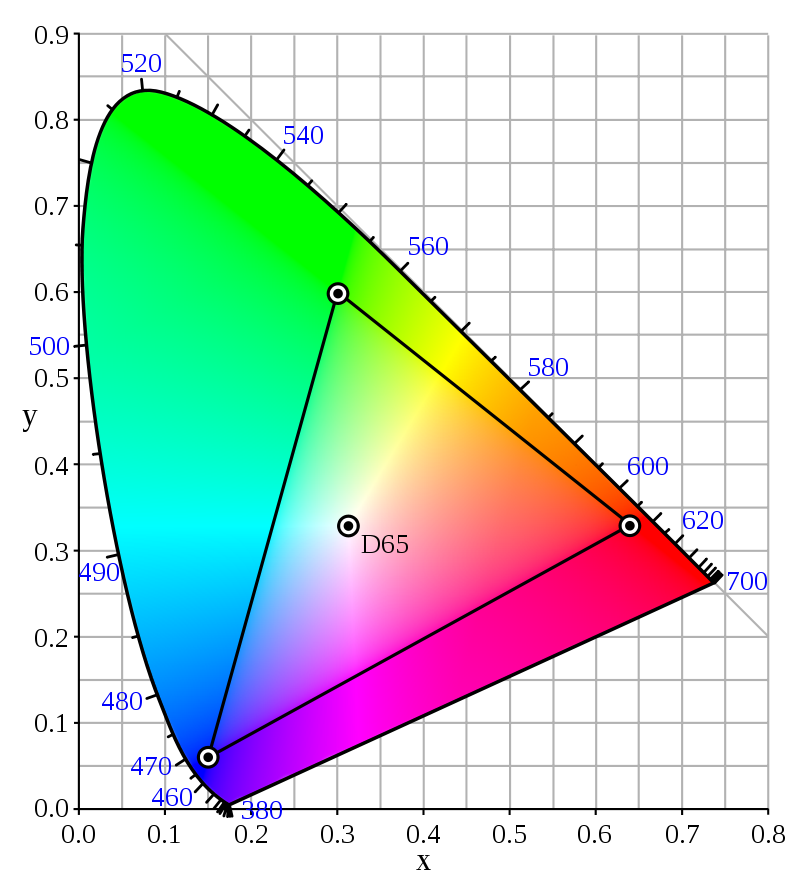
\includegraphics[width=0.5\textwidth]{abb11} 
	\caption{HD Farbraum}
\end{figure}
\subsection{Farbabtastung}
Bei der Farbabtastung handelt es sich um eine Komprimierung von  der Übertragung der Signale. Da ein unkomprimiertes Signal eine zu große Bandbreite in Anspruch nehmen würde, muss das Signal komprimiert werden. Dafür wird die Farbabtastung in Betracht gezogen. Da das menschliche Auge die Helligkeitskontraste besser auflöst als die Farbkontraste, wird bei der Farbabtastung die Helligkeit, oder Luminanz, mit der vollen Datenbreite zur Verfügung gestellt, die Farbinformation wird jedoch reduziert. Daraus ergibt sich dann ein voll aufgelöstes Signal mit der Farbabtastung von 4:4:4. Ein bereits komprimiertes Signal hat eine Farbunterabtastung von 4:2:2 oder 4:2:0 oder von 4:1:1.\footnote{\label{}vgl. Jörg Jovy, 2017, S. 114}
\paragraph[4:2:2]{4:2:2\protect\footnote{\label{}vgl. https://www.itwissen.info/Farb-Subsampling-color-subsampling.html [Zugriff: 18.03.2018]}}
\leavevmode \\
Bei der Farbunterabtastung von 4:2:2 wird bei jedem Pixel der Helligkeitswert abgetastet, wobei der Farbwert nur bei jedem zweiten Pixel abgetastet wird. 
\paragraph{4:2:0}
\leavevmode \\
\textit{"Beim Subsampling von 4:2:0, erfolgt die Abtastung der Chrominanzsignale für jeweils vier quadratisch angeordnete nebeneinander liegende Pixel. Wie bei den anderen Subsampling-Verfahren auch, wird das Luminanzsignal bei jedem Pixel abgetastet."} \footnote{\label{}https://www.itwissen.info/Farb-Subsampling-color-subsampling.html [Zugriff: 18.03.2018]}
\paragraph{4:1:1}
\leavevmode \\
Bei der Farbunterabtastung von 4:1:1 werden die Chrominanzsignale bei jeder vierter Abtastung abgetastet.
\begin{figure}[H]
	\centering
	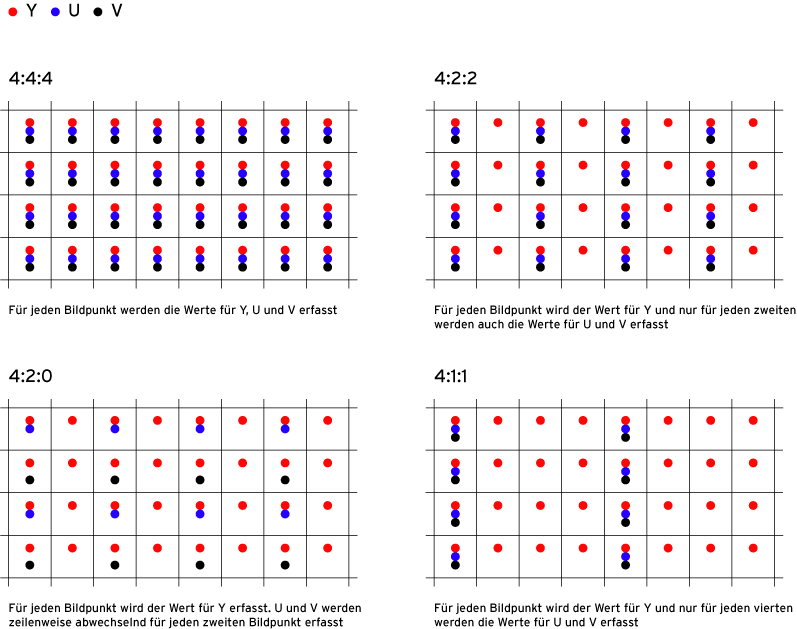
\includegraphics[width=1.0\textwidth]{abb15} 
	\caption{Farbabtastung}
\end{figure}
\section{Weißabgleich}
Bevor man ein Bild schießt, oder ein Video dreht, führt man einen Weißabgleich durch. Dabei wird zwischen manuellen und automatischen Weißabgleich unterschieden. Der Weißabgleich "misst die im Moment herrschende Farbtemperatur des Lichts." Die Farbtemperatur wird in Kelvin angegeben. Eine Kerze hat eine sehr rötliche und warme Farbstimmung mit einer Farbtemperatur von 1.500 Kelvin, wohingegen das Tageslicht neutral wirkt und eine Farbtemperatur von 5.000 bis 6.000 besitzt. Um den Weißabgleich manuell abzustimmen, wird ein weißes Blatt Papier vor die Kamera gehalten, und somit kann der Weißabgleich eingestellt werden. Das weiße Blatt Papier ist jedoch nur ein Hilfsmittel. Optimal wäre, eine professionelle Graukarte zu verwenden. Das Problem mit dem Papier ist, dass es optische Aufheller, die den Blauanteil erhöhen, besitzt. Das heißt, da die Kamera fälschlicherweise den zu hohen Blauanteil korrigiert, wird das Bild schlussendlich leicht gelbstichig. 
\section{Kameramodelle}
\subsection[DSLR Kamera - Aufbau]{DSLR Kamera - Aufbau\protect\footnote{\label{}vgl. http://bit.ly/2pnpDgL [Zugriff: 18.03.2018]}}
DSLR bedeutet Digital Single Lens Reflex und sind Spiegelkameras mit digitalem Aufnahme Sensor. Beispiele für eine Spiegelreflexkamera sind die Canon EOS 60D oder die Canon EOS 70. In der folgenden Abbildung wird der Aufbau einer DSLR Kamera dargestellt. Wie man in der Abbildung sehen kann, geht das Licht zuerst durch die Linse des Objektivs (1). Anschließend trifft das Licht auf den Schwingspiegel (2), welcher das Licht auf die Mattscheibe (5) reflektiert. Daraufhin verkleinert es die Sammellinse (6) auf die Größe des Suchers. Da das Bild noch spiegelverkehrt ist, spiegelt es das Pentaprisma (7) und kann so im Sucher (8) dann angezeigt werden. "Wenn man nun den Auslöser betätigt, klappt der Spiegel nach oben und gibt den Weg zum Schlitzverschluss (3) frei."\footnote{\label{}http://bit.ly/2pnpDgL [Zugriff: 18.03.2018]} Anschließend öffnet sich dieser Verschluss und das Licht fallt auf den Sensor (4). Zum Schluss wird das Bild dann abgespeichert.
\begin{figure}[H]
	\centering
	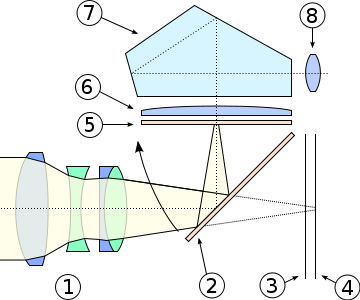
\includegraphics[width=0.6\textwidth]{abb13} 
	\caption{Aufbau einer DSLR Kamera}
\end{figure}
\subsection[Canon EOS 60D]{Canon EOS 60D\protect\footnote{\label{}vgl. http://bit.ly/2pnrmmy [Zugriff: 16.03.2018]}} Die Canon EOS 60D DSLR (Digital Single Lens Reflex) Kamera bietet einen 18 Megapixel APS-C CMOS Sensor mit einer Größe von 22,3 mm x 14,9 mm. Die Spiegelreflexkamera nimmt mit Full HD (1920 x 1080) auf, wobei standardgemäß mit 25 Bildern pro Sekunde aufgenommen wird. Die Auflösung wird meistens mit 1080p gekennzeichnet, wobei das p für progressive steht, also für die Vollbilder.
\subsection[Canon EOS 70D]{Canon EOS 70D\protect\footnote{\label{}vgl. http://bit.ly/2IxVmF2 [Zugriff: 16.03.2018]}} Die Canon EOS 70D bietet einen minimal größeren Sensor im Gegensatz zu der Canon EOS 60D. Die Größe des Sensors der Canon EOS 70D beträgt 22,5 mm x 15,0 mm. Die Sensorgröße einer Kamera ist entscheidend, da folgendes gilt: "Je kleiner der Sensor, desto geringer sind die Möglichkeiten, mit einer definierten Schärfentiefe zu arbeiten."
\footnote{\label{} Jörg Jovy, 2017, S. 136} Die Canon EOS 70D nimmt ebenfalls mit Full HD auf, wobei zu beachten ist, dass sie zusätzlich die Möglichkeit bietet, mit Intra-Frame oder Inter-Frame aufzunehmen. Bei Intra- oder Inter-Frames wird jedes Einzelbild komprimiert, das heißt, es kann auf jedes einzelne Bild zugegriffen werden
\footnote{\label{}vgl. https://www.univie.ac.at/video/grundlagen/intraframe.htm [Zugriff: 17.03.2018]}, was sich in der Post Production positiv widerspiegelt, da man keine Gruppen aus Bildern bearbeiten muss, sondern im Notfall jedes einzelne Bild bearbeiten kann. Weiters spielt bei der Wahl der richtigen Kamera, der Cropfaktor eine wichtige Rolle. "Je kleiner ein Sensor ist, desto kleiner ist auch der Bildwinkel des Objektivs."
\footnote{\label{}Jörg Jovy, 2017, S. 136} Das bedeutet, dass die Abbildungsfläche beschnitten wird, was einen engeren Bildausschnitt liefert und somit ein vergrößertes Bild darstellt. Was bei DSLR Kameras zu beachten ist, ist das sie einen Cropfaktor von 1,6 besitzen. So verhält sich durch den Cropfaktor von 1,6 ein Normalobjektiv mit 50mm Brennweite, wie ein leichtes Teleobjektiv mit 80mm Brennweite. 
Da die Canon EOS 70D einen minimal größeren Sensor besitzt, und die Möglichkeit bietet, mit Intra-Frames aufzunehmen, wurde die Canon EOS 70D DSLR Kamera für alle Aufnahmen verwendet.
\subsection[Objektive]{Objektive\protect\footnote{\label{}vgl. Jörg Jovy, 2017, S. 138f.}}
Die Brennweite eines Objektivs legt den Bildausschnitt fest. Die Brennweite wird in Millimeter angegeben und sagt aus, ob es sich um ein Normal-, Tele-, oder ein Weitwinkelobjektiv handelt.
Anhand der folgenden Abbildung kann man gut erkennen, dass ab 10 mm bis 24 mm Weitwinkelobjektive zum Einsatz kommen. Ein Normalobjektiv erkennt man daran, da es eine Brennweite von 50 mm besitzt und hat somit einen Bildwinkel mit 46$^\circ$ hat. Teleobjektive finden ihren Einsatz bei 80 mm bis 200 mm. Anhand der Abbildung kann man gut den Unterschied zwischen der Brennweite von 10 mm und einem Bildwinkel mit 130$^\circ$ , und einem Objektiv mit einer Brennweite von 200 mm mit 12$^\circ$ Bildwinkel erkennen. 
\begin{figure}[H]
	\centering
	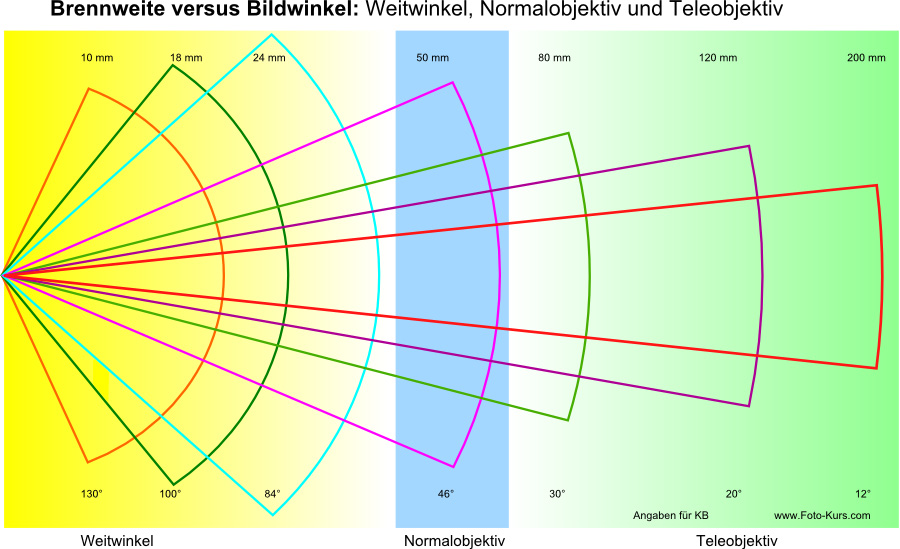
\includegraphics[width=0.7\textwidth]{abb1} 
	\caption{Brennweite und Bildwinkel}
\end{figure}
\begin{itemize}
	\item Normalobjektiv\footnote{\label{}vgl. Jörg Jovy, 2017, S. 196f.}
		\begin{itemize}
		\item Das Normalobjektiv entspricht im Grunde dem menschlichen Blickwinkel, und wird meist als natürlich empfunden. 
		\end{itemize}
	\item Weitwinkel
		\begin{itemize}
		\item Wie man auf der obigen Abbildung sehen kann, haben Weitwinkelobjektive einen breiten Bildwinkel, somit sieht man mehr vom Bild. 
		\end{itemize}
	\item Teleobjektiv
		\begin{itemize}
		\item Teleobjektive nehmen Objekte mit einem kleinen Blickwinkel aus großer Entfernung auf. Teleobjektive haben daher einen eher kleinen Schärfentiefenbereich, was sich beispielsweise für Interviews schlecht eignet. 
\end{itemize}
\end{itemize}
\section[Beleuchtung]{Beleuchtung\protect\footnote{\label{}vgl. Jörg Jovy, 2017, S. 236ff.}}
In der Videografie wird die Belichtungszeit in der Bildrate vorgegeben, wohingegen sie in der Fotografie zwischen mehreren Stunden und wenigen Sekunden liegen kann.
Die richtige Belichtungszeit kann man sich mit folgender Formel berechnen: Belichtungszeit = 1: Framerate x 2. Nimmt man nun mit 25 Bildern pro Sekunde auf, ergibt sich eine Belichtungszeit von 1:50 = 1/50 s. Würde man die Belichtungszeit verkürzen, z.B. auf 1/125 s, dann würde das Bild zwar schärfer werden, aber dann würde die Gefahr bestehen, dass der sogenannte Moir\'{e} Effekt eintritt. Der Moir\'{e} Effekt ist ein Bildfehler, der bei bewegten Bildern ein Flimmern erzeugt. Bei dem "Effekt" liegen feine Muster oder Raster in einem gegeneinander verschobenen Winkel übereinander, welche sich gegenseitig beeinflussen. 
\begin{figure}[H]
	\centering
	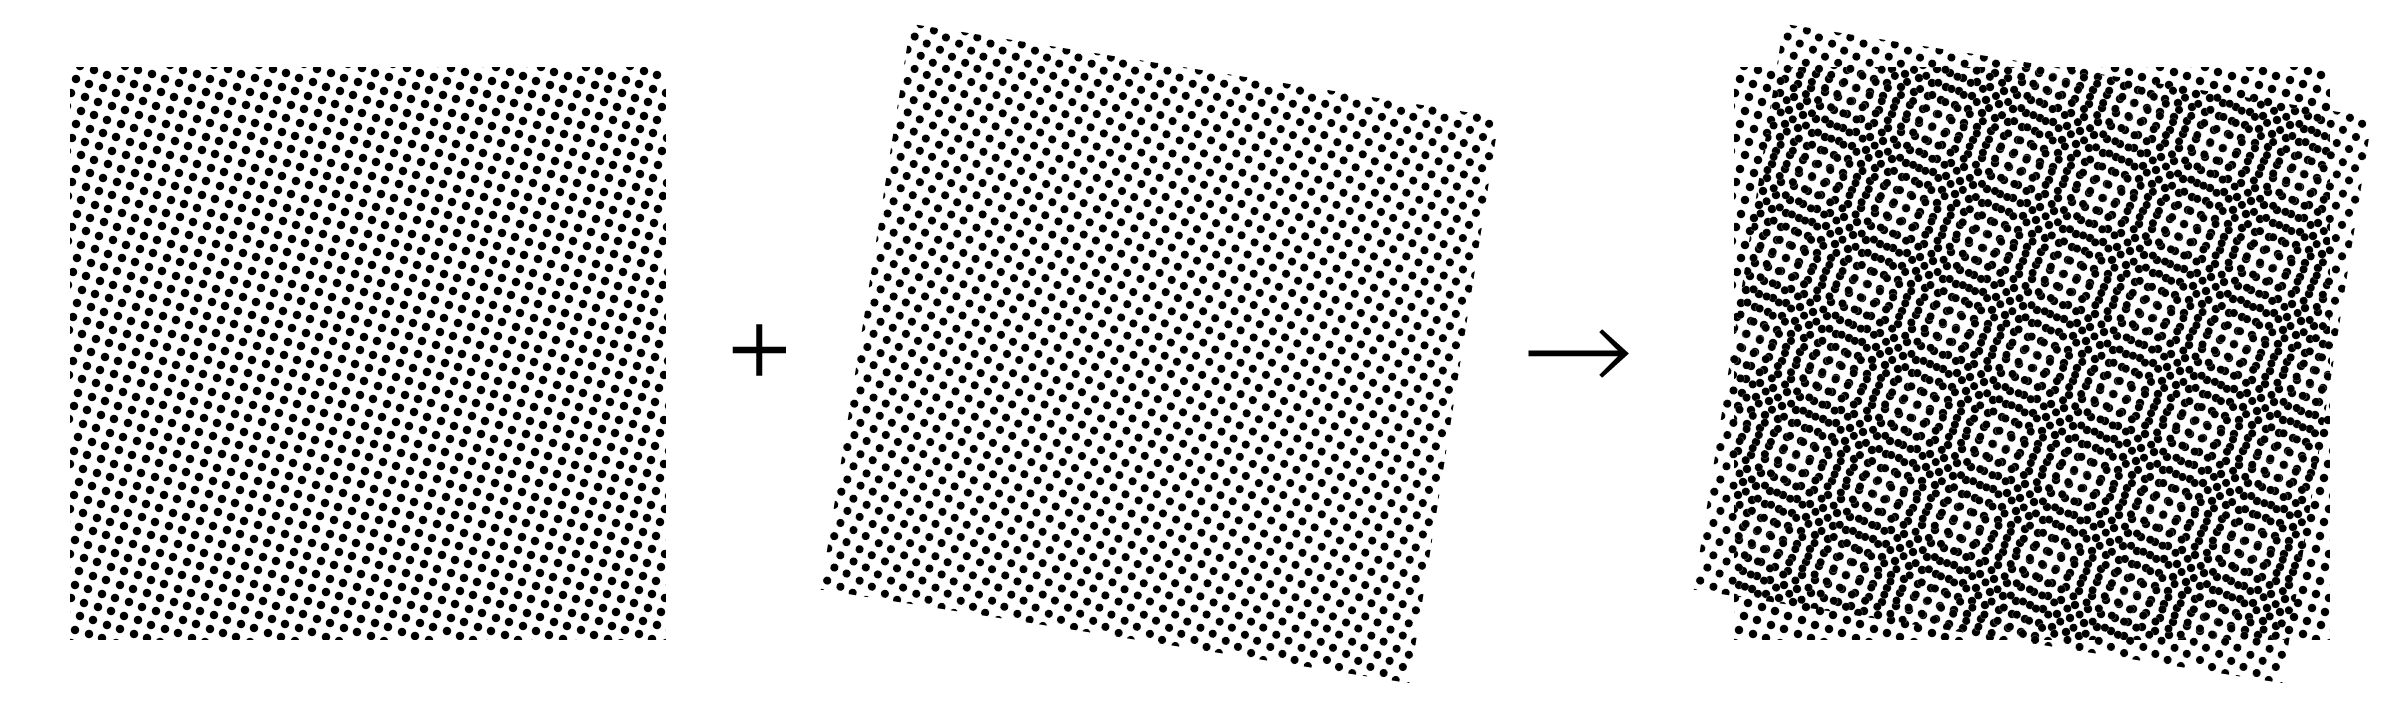
\includegraphics[width=0.8\textwidth]{abb2} 
	\caption{Moir\'{e}-Effekt}
\end{figure}
Bei der Beleuchtung muss man drei Positionen von den Lichtquellen der Belichtung unterscheiden. Das Licht, das von vorne auf den Gegenstand kommt, nennt man Gegenlicht. Das Licht, das von der Seite kommt, wird als Streiflicht bezeichnet, und als drittes Licht wird das Auflicht verwendet, welches von hinten auf das Objekt scheint.
\begin{figure}[H]
	\centering
	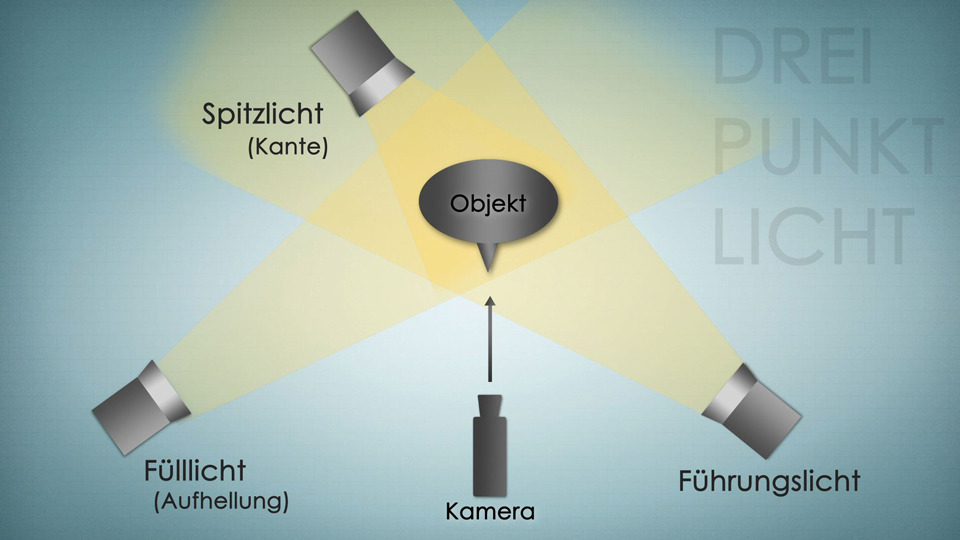
\includegraphics[width=0.8\textwidth]{abb3} 
	\caption{Zusammenspiel der Lichter}
\end{figure}
Wie man auf der Abbildung 6.6 erkennen kann, ist es wichtig, wie die Lichter im Verhältnis zueinander stehen. Das Führungslicht, oder auch Hauptlicht genannt, dient dazu, die Szene generell aufzuhellen. Durch die Verwendung des Führungslichts entstehen Schatten, die wiederrum mit dem Fülllicht reduziert werden. Um den Gegenstand auch optisch vom Hintergrund abzuheben, kommt das sogenannte Spitzlicht zum Einsatz. \footnote{\label{}vgl. http://www.filmmachen.de/tipps-und-tricks/licht/3-punkt-beleuchtung [Zugriff: 17.03.2018]}
\section{Mikrofone}
\subsection{Richtcharakteristik}
\textit{"Die Richtcharakteristik definiert, aus welcher Richtung das Mikrofon den Schall besonders empfindlich aufnimmt. Stark vereinfacht gesagt: Aus welcher Richtung aufgenommen wird."}\footnote{\label{}https://www.delamar.de/mikrofon/richtcharakteristik-mikrofon-22647/ [Zugriff: 17.03.2018]} 
\subsubsection[Kugelcharakteristik]{Kugelcharakteristik\protect\footnote{\label{}vgl. https://www.delamar.de/mikrofon/richtcharakteristik-mikrofon-22647/ [Zugriff: 17.03.2018]}}
Bei der Kugelcharakteristik wird der Schall von allen Richtungen aufgenommen, das heißt es wird von keiner bevorzugten Richtung aufgenommen. Das Problem, was dadurch entsteht, ist, dass die Rückkoppelanfälligkeit sehr hoch ist, wodurch Mikrofone mit einer Kugelcharakteristik schlecht für Bühnen geeignet sind. 
\begin{figure}[H]
	\centering
	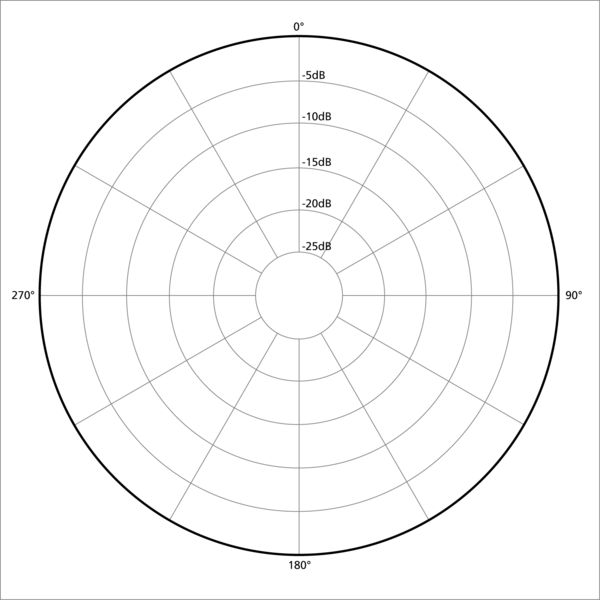
\includegraphics[width=0.4\textwidth]{abb4} 
	\caption{Kugel}
\end{figure}
\subsubsection{Nierencharakteristik}
Die Niere nimmt, im Gegensatz zur Kugelcharakteristik, aus einer bevorzugten Richtung auf. Wo, der Schall bei der Kugel von allen Seiten aufgenommen wird, wird er bei der Niere nur von einer Seite aufgenommen, meistens von vorne. Der Schall wird von den Seiten nur sehr leise bis gar nicht aufgenommen. Der Vorteil, der Niere ist, dass sie rückkopplungsfester, als die Kugel ist und sie so auch beispielsweise bei Konzerten verwendet werden kann. Der Nachteil der Niere ist der sogenannte Nachbesprechungseffekt. Das bedeutet: "Ab einer gewissen Nähe der Schallquelle werden die tieffrequenten Anteile dominanter."\footnote{\label{}https://www.delamar.de/faq/nahbesprechungseffekt-34021/ [Zugriff: 17.03.2018]}
\begin{figure}[H]
	\centering
	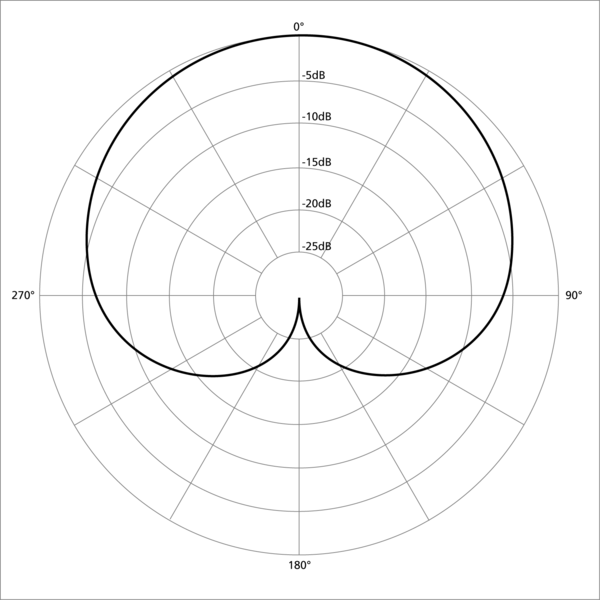
\includegraphics[width=0.4\textwidth]{abb5} 
	\caption{Niere}
\end{figure}
\subsubsection{Keule/Superniere}
Keule beziehungsweise Superniere sind Charakteristiken, die von der Niere abgeleitet sind. Die Fläche der Keule ist im Gegensatz zu der Niere etwas schmaler. Das hat die Auswirkung, das von den Seiten weniger aufgenommen wird. Dadurch sind Mikrofone mit einer Keule oder Superniere hinten empfindlicher. "Dennoch haben sie die höchste Rückkopplungsfestigkeit."\footnote{\label{}https://www.delamar.de/mikrofon/richtcharakteristik-mikrofon-22647/ [Zugriff: 17.03.2018]}
\begin{figure}[H]
	\centering
	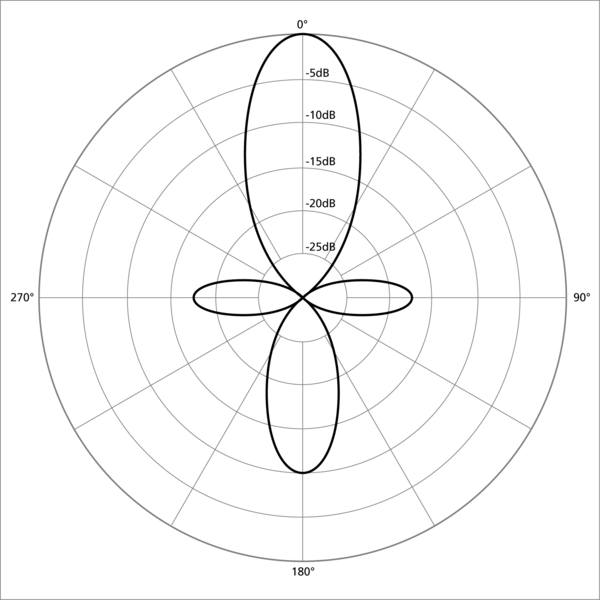
\includegraphics[width=0.4\textwidth]{abb6} 
	\caption{Keule}
\end{figure}
\subsubsection{Acht}
Die sogenannte Achtcharakteristik nimmt den Schall von vorne und hinten auf, jedoch nur minimal von den Seiten. Diese Charakteristik hat die Verwendung bei der M/S-Stereofonie. 
\begin{figure}[H]
	\centering
	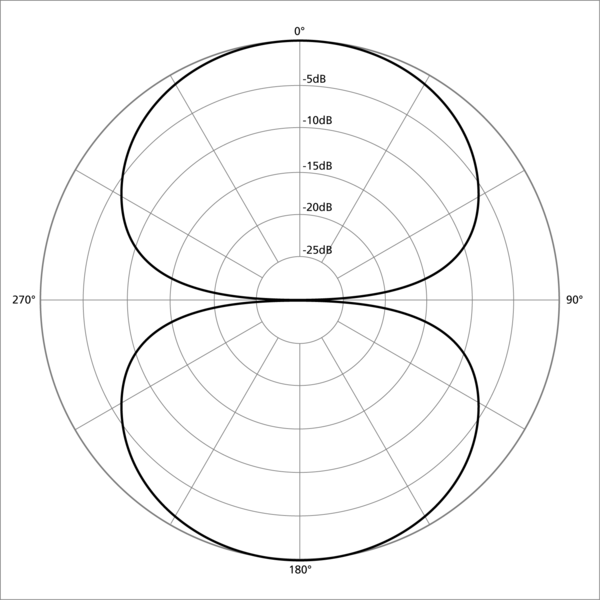
\includegraphics[width=0.4\textwidth]{abb7} 
	\caption{Acht}
\end{figure}
\subsection{Kondensatormikrofon}
"Ein Kondensatormikrofon wandelt Schall in ein elektrisches Signal."\footnote{\label{}https://www.delamar.de/faq/kondensatormikrofon-34728/ [Zugriff: 17.03.2018]} Bei einem Kondensatormikrofon treffen die Schallwellen zuerst auf die Membran, was eine leitende Folie ist, die mit Gold bedampft ist. Dies verbessert die  Leitfähigkeit des Mikrofons, was die Luftdruckschwankungen in mechanische Schwingungen umwandelt.\footnote{\label{}vgl. https://www.delamar.de/faq/kondensatormikrofon-34728/ [Zugriff: 17.03.2018]} Anschließend wird sie in elektrische Spannung umgewandelt und über die XLR-Buchse wieder ausgegeben. 
\begin{figure}[H]
	\centering
	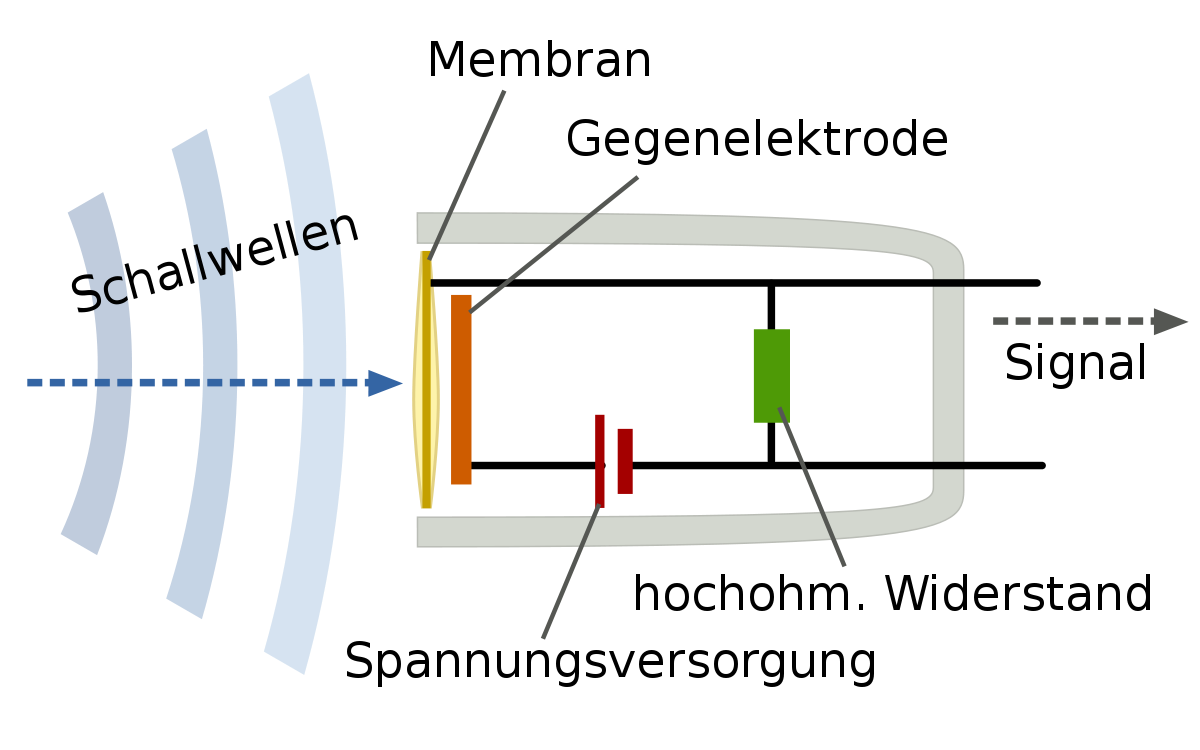
\includegraphics[width=0.6\textwidth]{abb8} 
	\caption{Kondensatormikrofon}
\end{figure}
\subsection{Dynamisches Mikrofon}
\textit{"Bei diesem Mikrofontyp wird das Signal durch elektromagnetische Induktion erzeugt. Kurz: Der Schall trifft auf die Membran des Mikrofons und regt sie zu mechanischen Schwingungen an, die durch eine mit der Membran verbundene Spule in elektrische Spannung umgewandelt werden. Und diese kommt dann aus der (XLR-)Buchse des Mikrofons."}\footnote{\label{}https://www.delamar.de/faq/dynamisches-mikrofon-34718/ [Zugriff: 17.03.2018]}
\begin{figure}[H]
	\centering
	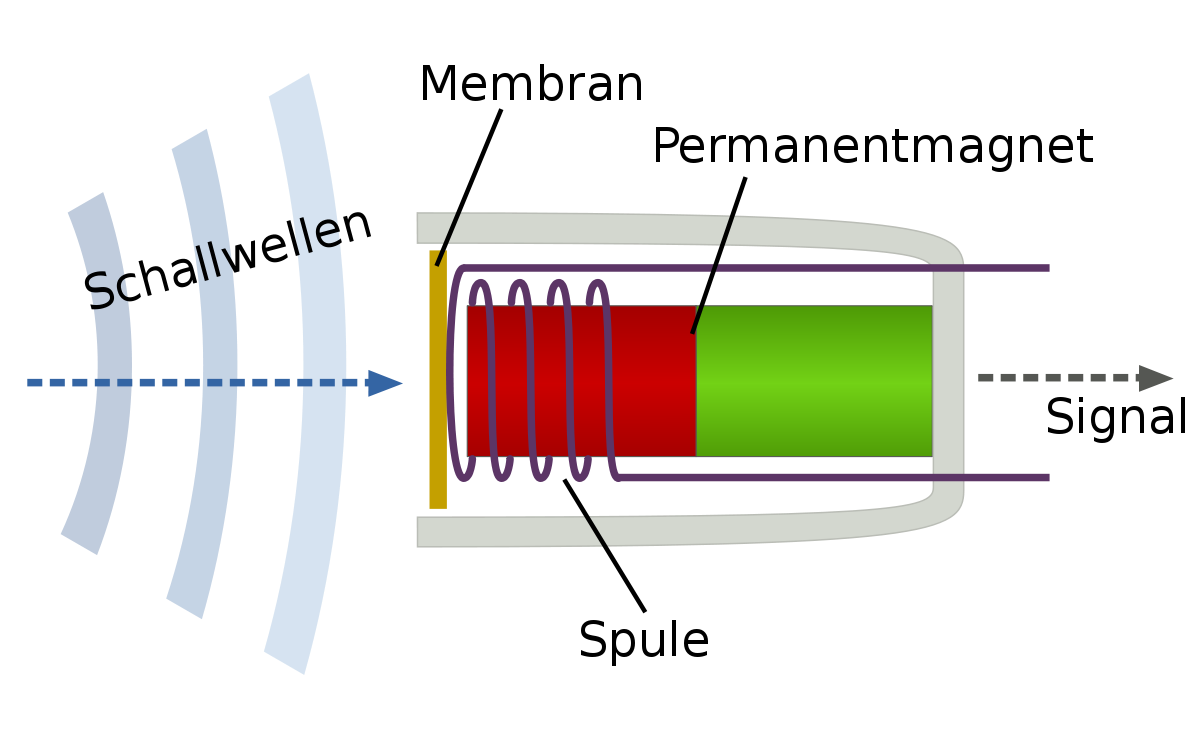
\includegraphics[width=0.6\textwidth]{abb9} 
	\caption{Dynamisches Mikrofon}
\end{figure}
\section[Planung und Vorbereitung]{Planung und Vorbereitung\protect\footnote{\label{}vgl. Jörg Jovy, 2017, S. 50ff.}}
Für die Planung eines Videos benötigt man meistens viel Zeit, um auch ein gutes Ergebnis zu erzielen. Bevor es an das bekannte Drehbuch geht, muss man vorerst noch drei andere Schritte berücksichtigen, nämlich die sogenannte Logline, das Expos\'{e} und das Treatment. Erst nach diesen Schritten ist es sinnvoll das Drehbuch zu schreiben. 
\subsection{Logline}
Die Logline ist vereinfacht gesagt, die Idee zum Film oder zum Video. Die Logline besteht meistens nur aus einem Satz und soll nur einen groben Überblick über den Film oder des Videos preisgeben. 
\subsection{Expos\'{e}}
Das Expos\'{e} besteht meist nur aus ein paar Skizzen, wobei folgende Themen behandelt werden: das Thema selbst, die Besonderheiten des Videos oder Films, die Protagonisten, Drehorte und sonstige Herausforderungen. Das Expos\'{e} soll den Mitarbeitern dienen, weitere Entscheidungen leichter zu treffen.
\subsection{Treatment}
Das Treatment ist mehr oder weniger der Vorgänger des Drehbuchs. Ein Treatment beinhaltet schon kurze Dialoge zu bestimmten Szenen und eine szenengenaue Auflösung zum Film oder Video.
\subsection{Drehbuch}
Das Drehbuch ist, im Vergleich zum Treatment, komplett ausgearbeitet, das heißt, es liegt ein kompletter Produktionsleitfaden vor, wobei jede Szene ausgearbeitet ist. Weiters wenden wichtige Einstellungen in Bildszenen dargestellt. Adobe bietet die kostenlose Software \textit{Story} an, mit der man Drehbücher erstellen kann. 
\subsection{Storyboard}
Ein Storyboard ist eine visualisierte Veranschaulichung von dem Konzept, das man sich zuvor überlegt hat.\footnote{\label{}vgl. https://www.e-teaching.org/didaktik/konzeption/inhalte/storyboard [Zugriff: 16.03.2018]}Um die korrekte Ausführung der Videos zu gewährleisten, wurden sogenannte Storyboards angefertigt. Diese wurden mit der Online Plattform "Storyboard That"\footnote{\label{}https://www.storyboardthat.com/ [Zugriff: 16.03.2018]} erstellt und schließlich als PDF - Format exportiert.
Im Storyboard wurden die Szenen bildlich dargestellt, was das Team im weiteren Verlauf unterstützte, da es dadurch grobe Fehler vermeiden konnte.
Das Online - Tool ermöglichte es zwischen verschiedensten Szenen, Charakteren und Kategorien auszuwählen, wodurch vereinfacht, verschiedenste Szenen dargestellt werden konnten. 
\begin{figure}[H]
\begin{center}
	\fbox{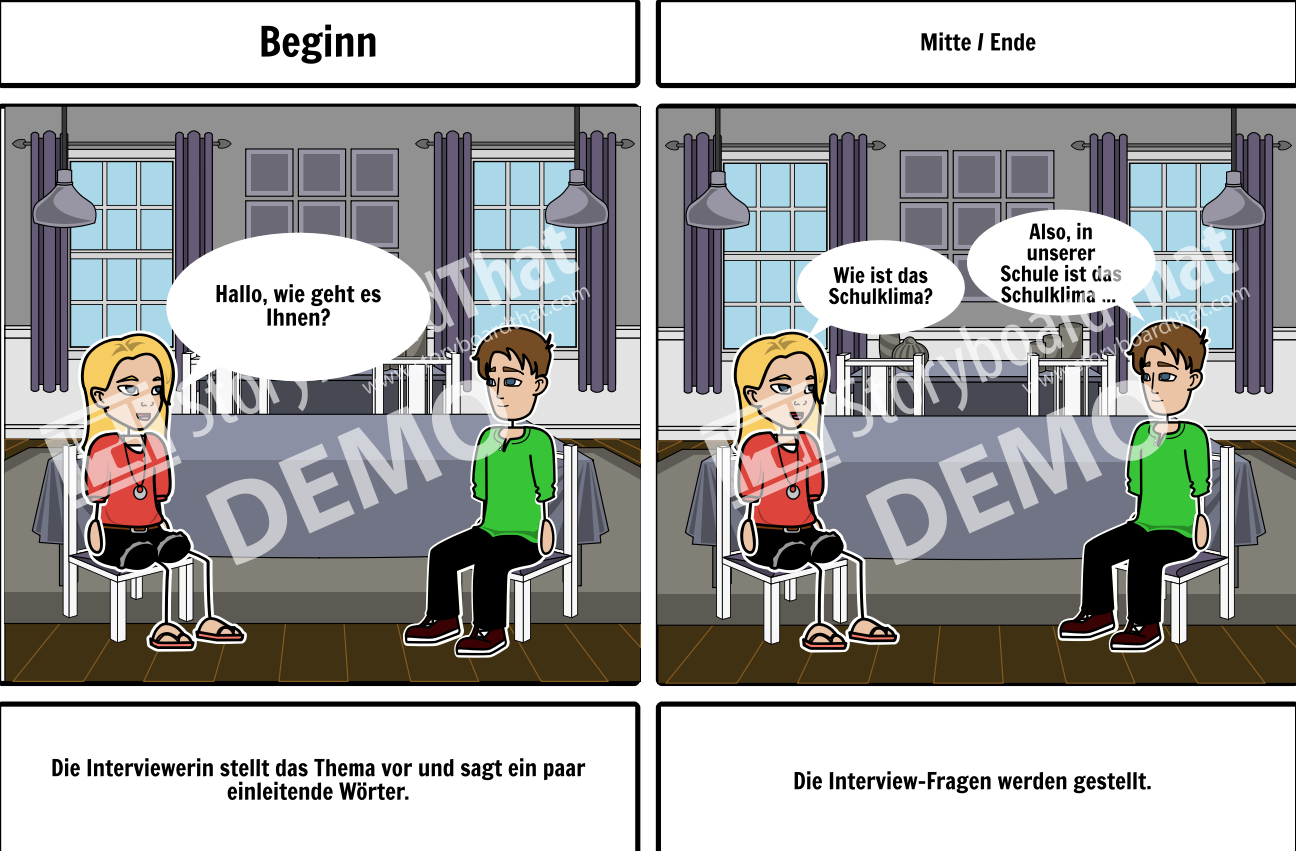
\includegraphics[scale=0.30]{abb10}}
	\caption{Storyboard}
\end{center}
\end{figure}
\section{Setting}
Beim Aufbau des Sets wurde auf das Drehbuch und das Storyboard referenziert. Hierbei wurde auch die Location berücksichtigt, da für den Aufbau eines Videos mit Greenscreen ein anderes Set von Nöten war, als bei einem Video am Gang in der Schule. Weiters musste überlegt werden, wie die Kameras und Lichter platziert werden müssen. Bevor es zum eigentlichen Dreh kam, wurden die jeweiligen Drehs im Vorhinein ausreichend getestet, um später beim wirklichen Dreh, Fehler zu vermeiden. Weiters wurden zusätzlich verschiedene Mikrofone getestet, um für die jeweilige Situation das optimale Mikrofon zu verwenden.
\section{Post Production}
\subsection{Aufnahmeformate}
Bei der Auswahl des Aufnahmeformates muss man sich im Klaren sein, mit welchem Codec man aufnehmen möchte. Hierbei muss man zwischen Codecs und Containern unterscheiden. Container, welche den Videostream mittels eines Codecs digitalisieren, speichern die Videodaten auf dem Speicherchip. Audio Video Interleave (AVI), QuickTime (MOV) oder Moving Pictures Expert Groups (MPEG) sind zum Beispiel solche Containerformate. Ein Codec wandelt analoge Bilder in digitale Datenströme um. Bei der Codierung wird das Bild komprimiert, was wiederum mehr Speicherplatz zur Verfügung stellt. DivX, QuickTime H.264, Apple ProRes, Panasonic AVC-Intra oder Avid DNxHD sind typische Codecs. 
\paragraph{MPEG}
\leavevmode \\
"MPEG ist ein standardisiertes Kompressionsverfahren, das sich speziell zur Datenreduktion von Bewegtbildern eignet."\footnote{\label{}https://www.film-tv-video.de/term-word/mpeg/ [Zugriff: 26.03.2018]} MPEG lässt dem Gerätehersteller freie Wahl, bezüglich der Entscheidung der Datenerzeugung. Jedoch legt MPEG das Datenformat und die Dekodierung vor. Was noch beachtet werden muss, ist, dass schlussendlich ein normgerechter MPEG-kodierter Datenstrom entstehen muss, der mit einem MPEG-Decoder gelesen und wiedergegeben werden kann. Bei dem MPEG Standard setzen sich die Einzelbilder einer Videosequenz aus einer Folge von I-, B- und P-Frames zusammen. Diese Aufeinanderfolgung wird Group of Pictures, kurz GOP, genannt. Eine Group of Pictures muss mindestens ein I-Frame enthalten. I-Frames sind Indexbilder, welche die wichtigsten Bildinformationen enthalten. "B-Frames sind  bidirektionale Bilder, also Frames, die nur die Unterschiede eines Bildes zum vorhergehenden oder folgenden Bild beinhalten."\footnote{\label{}https://www.film-tv-video.de/term-word/mpeg/ [Zugriff: 26.03.2018]} P-Frames sind Predicted Frames. Predicted Frames werden aus den vorherigen I-Frames berechnet.
\paragraph{MP4}
\leavevmode \\
MP4 ist das Containerformat von MPEG. 
\paragraph{QuickTime}
\leavevmode \\
\paragraph{AVI}
\leavevmode \\
\subsection{Kompressionsverfahren}
Bei der Bildkompression werden die Bildinformationen in 4x4, 8x8 oder 16x16 Pixeln zusammengefasst. "In einzelnen Bildern und zwischen aufeinanderfolgenden Bildern werden dann sich wiederholende Daten identifiziert." Nun können die wiederholenden Informationen gefiltert und weggelassen werden. Bei dem MPEG-2 Container wird zum Beispiel nur jedes zwölfte Bild komplett gespeichert, wobei bei den anderen Bildern nur Teile beziehungsweise Veränderungen gespeichert werden. Da nur jedes zwölfte Bild komplett gespeichert wird, ist das Risiko enorm groß, dass Artefakte, also Bildfehler, entstehen können. Die sogenannten Artefakte entstehen bei der Umwandlung von digitalen Bildern in analoge Bildsignale. 
\subsection{Schnittprogramme}
\paragraph{Lightworks}
\leavevmode \\
Lightworks ist ein lizenzfreies Videoschnittprogramm, das auf Windows, Linux und auf IOS Betriebssystemen verwendet werden kann. Lightworks bietet nicht nur die freie Version, sondern auch eine Pro Version. Die freie Version bietet dem User eine Vielzahl an importierbaren Formaten, wie zum Beispiel Apple Pro Res, AVC-Intra 50, MPEG-2 Long GOP und vieles mehr. Weiters kann man in Lightworks seine Videos mit dem Codec H.264 mit der Auflösung 1280x720p kodieren. 
\paragraph{Adobe Premiere Pro}
\leavevmode \\
Adobe Premiere Pro ist eine kostenpflichtige Software, welche aber eine Vielzahl von Funktionalitäten bietet. 
\subsection{Schnitt}

\section{Interview mit dem Abteilungsvorstand}
\subsection{Idee}
Die Intention des Interviews mit dem Abteilungsvorstand Dr. Hager war es, Interessenten allgemeine Informationen über die Schule näher zu bringen. 
\section{Tag der offenen Tür}
\subsection{Idee}
Das Tag der offenen Tür Video dreht sich um die Interessenten, die sich die Schule am Tag der offenen Tür angeschaut haben. Hierbei wurden Fragen, wie: "Wie ist dein erster Eindruck von der Schule", oder "Kannst du dir vorstellen dich hier anzumelden", gestellt. Weiters redet am Ende des Videos ein Lehrer über die Schule und erklärt, ob eine HTL oder eine AHS geeigneter wären.
\section{Video mit einem Absolvent}
\subsection{Idee}
Bei dem Video beziehungsweise Quiz mit dem Absolventen und dem Schüler der zweiten Klasse geht es darum, dass dem Absolventen und dem Schüler Fragen gestellt werden, wobei sie 45 Sekunden Zeit haben diese zu beantworten. Derjenige, der die Frage falsch beantwortet, muss ein Jelly-Bean essen, wobei man nicht weiß, ob es ein gutes oder ein schlechtes ist. Die Intention dieses Videos ist es zu zeigen, dass die Medientechnik ein enorm großer Bereich ist bei dem man nicht alles erlernen kann. So spezialisiert sich jeder Schüler meist auf ein Gebiet, das er dann auch dementsprechend gut kann. Was jedoch zu beachten ist, ist, dass die Schüler dennoch die Grundlagen der anderen Gebieten lernen und auch können.
\section{Herausforderungen}
\subsection{Interview mit dem Abteilungsvorstand}
Das Problem bei dem Dreh, mit dem Interview des Abteilungsvorstandes, war, dass die Blende zu weit geöffnet war, und so es nicht möglich war die Schärfentiefe zu erzeugen. Die Schärfentiefe wird durch die Blende, der Sensorgröße und der Brennweite definiert. Da man an der Sensorgröße nach dem Kauf der Kamera nichts mehr ändern kann, muss man sich mit den anderen zwei Bereichen auseinandersetzen. Je weiter die Blende geschlossen ist, desto mehr Schärfentiefe kann erzielt werden. Je offener die Blende ist, umso weniger Schärfentiefe hat man. Die Brennweite beeinflusst die Schärfentiefe insofern, da je größer die Brennweite ist, also je näher man an ein Objekt heranzoomt, desto unschärfer wird der Hintergrund. 
Wie man in der Abbildung sehen kann, befinden sich im Hintergrund zu viele Störfaktoren, die aufgrund der fehlenden Schärfentiefe gut erkennbar sind, und dem Zuseher vom eigentlichen Bild ablenken würden. 
Das Programm Adobe Premiere Pro ermöglicht es mittels einer Maske einen Maskenpfad zu setzen, den man später auch "bewegen" kann. Das bedeutet, dass sich die Maske Frame für Frame fortbewegt und sich anpasst. Jedoch war dies hier nur begrenzt möglich, da sich der Hintergrund nicht sonderlich abhebt, und so die Maske sich nicht mitbewegen konnte. Der Maskenpfad musste schließlich bei manchen Frames manuell nachbearbeitet werden.
Man kann beim Erstellen der Maske entscheiden, ob man die Maske mittels einer Ellipsen Form, einer Rechteck Form oder mit einem Zeichenstift erzeugen will. Bevor man die Maske zeichnet, wählt man den Effekt aus, mit dem man arbeiten will. Im folgenden Fall, war es den Hintergrund unscharf zu zeichnen, also war die Verwendung eines Weichzeichners nötig. Man zieht den gewünschten Effekt ins Schnittfenster und anschließend kann man das gewünschte Werkzeug auswählen, in dem Fall den Zeichenstift. Dies war deswegen notwendig, da man auch die Person auswählen musste, was mit einem Kreis oder Rechteck nicht möglich gewesen wäre. Hat man ein Werkzeug ausgewählt, kann man auch schon die Maske setzen. Adobe Premiere Pro bietet zusätzlich noch eine weiche Kante auf Masken anzuwenden. Dies ist deswegen von großer Bedeutung, da ansonsten der maskierte Bereich mit dem anderen nicht "verschmilzen" würde. Das heißt, man würde die harten Kanten zwischen den zwei Objekten deutlich erkennen. Die weiche Kante glättet den Maskenauswahlrahmen und ermöglicht einen schönen Übergang zwischen Maskenkante und dem anderen Bereich.
\subsection{Tag der offenen Tür Video}
Das Video des Tag der offenen Tür wurde am Gang in der Schule gedreht. Da unter anderem manche Lichter immer wieder aus und an gingen, waren oftmals andere Lichtverhältnisse vorhanden. Diese mussten in der Post Production ebenfalls nachbearbeitet werden. Bei der Bearbeitung der Farbe wurden die Lumetri Scopes Grafiken herangezogen. Diese dienten insofern gut, da man auf einen Blick gesehen hat, von welcher Farbe am meisten Information vertreten ist, und wo noch etwaige Farbinformation fehlt. Mithilfe des Vektorskops, Histogramms und des Waveform-Monitors konnte die Farbe korrigiert werden.
\paragraph{Vektorskop}
\leavevmode \\
"Das Vektorskop gibt Auskunft über die Farbverteilung im Bild."\footnote{\label{}buch} Auf dem Vektorskop sind die Grundfarben aus dem RGB und dem CMYK Farbraum abgebildet. Also: Rot, Grün, Blau, Cyan, Magenta, Yellow. Je weiter der Signalpunkt sich vom Zentrum entfernt, desto höher ist die jeweilige Farbsättigung. Hätte man ein Schwarz-Weiß-Bild würde man einen Punkt in der Mitte sehen.
\paragraph{Histogramm}
\leavevmode \\
Das Histogramm zeigt die Häufigkeitsverteilung von Helligkeit und Farbe, die im Bild vorkommt. Weiters zeigt das Histogramm, ob das Bild korrekt belichtet wurde. Das Histogramm geht von 0,0,0 für RGB Schwarz bis 255,255,255 für RGB Weiß. Die Schatten befinden sich beim Histogramm unten, also in Richtung 0,0,0, wobei man die Lichter oben, also in Richtung 255,255,255 findet.
\paragraph{Waveform-Monitor}
\leavevmode \\
Der Waveform-Monitor zeigt die Helligkeitsverteilung im Bild. Die Helligkeit wird als Häufigkeitsverteilung wiedergegeben, wobei 100\% Weiß einen Messwert von 100 IRE entsprechen. "IRE ist die international übliche Skalierung. 0 IRE entsprechen daher Schwarz. Mithilfe des Waveform-Monitors kann man einfach die sogenannten Lichter, Mitten und Tiefen einfach analysieren. 
\subsection{Video mit einem Absolvent}
Da beim Dreh des Videos der Schüler der zweiten Klasse etwas unschärfer war, war es nötig manuell nachzuschärfen. "Mit dem Effekt 'Scharfzeichner' kann der Kontrast an den Stellen mit Farbänderungen verstärkt werden." Jedoch sollte der Effekt sparsam eingesetzt werden, da es schnell unnatürlich wirken kann. Bei dem Video gab es nicht grobe Herausforderungen. Bei dem Video wurden jedoch verstärkt verschiedene Blenden eingesetzt, um es spannend und abwechslungsreich zu gestalten. 
\paragraph{Effektblenden}
\leavevmode \\
Die Effektblende wird als Gestaltungsmittel bezeichnet, mit der man einen Übergang von einem Ereignis zum anderen besser bildlich darstellen kann. Bei dem Quiz mit dem Absolventen und dem Schüler wurde einerseits die Effektblende "Wegschieben", als auch "Einzoomen \& Auszoomen" und "Filmblende" verwendet. Die Blende "Wegschieben" dient dazu von einem Bild,  also zum Beispiel von einer Antwort zur nächsten Frage überzugehen. Der "Einzoomen \& Auszoomen" Effekt wurde beim Einblenden der Antworten verwendet. Zuletzt wurde die "Filmblende" für das Einblenden der Punkte verwendet.
